\documentclass{standalone}
\usepackage{color}
\usepackage{tikz}
\definecolor{accent}{HTML}{00C853}
\definecolor{gray500}{HTML}{757575}

\usetikzlibrary{arrows}
\tikzstyle{vertice}=[circle, draw=black, fill=gray500, inner sep=1mm]
\begin{document}


\usepackage[backend=bibtex]{biblatex}
\usepackage[utf8]{vietnam}
\usepackage[T1]{fontenc}
\usepackage{inconsolata}
\bibliography{uni}
\renewcommand{\bibname}{Danh mục tài liệu tham khảo}
\nocite{*}

\newcommand{\abs}[1]{\left\lvert#1\right\rvert}
\everymath{\displaystyle}
\renewcommand{\qedsymbol}{$\blacksquare$}

\begin{document}
\pagenumbering{roman}\pagestyle{plain}
\pagestyle{fancy}
\lhead{\thepage}
\cfoot{}
\renewcommand{\footrulewidth}{0pt}
\begin{titlepage}
	\begin{minipage}[c]{4em}
		
\includegraphics[width=3em]{resources/bk.jpg}
	\end{minipage}
	\begin{minipage}[l]{\textwidth - 4em}
		{\Huge Trường Đại học Bách khoa Hà Nội\par}
		{\large Viện Toán ứng dụng và Tin học}
	\end{minipage}
	\vfill
	\vfill
	\begin{center}
		{\Large Tài liệu toán rời rạc}\par
		{\LARGE Một số khái niệm cơ bản trong lý thuyết đồ thị}\par
		\vfill
		{\large
			\begin{tabular}{rl}
				{ Giảng viên hướng dẫn}:&TS. Lê Chí Ngọc\\
				{ Sinh viên thực hiện:}& Nguyễn Đức Hùng\\
				{ Lớp học:} & TN Toán -- tin K62
			\end{tabular}
		}
		\vfill
		{\large Hà Nội, tháng 5 năm 2019}
	\end{center}
\end{titlepage}
\tableofcontents

\chapter{Một số khái niệm cơ bản}
\section{Đồ thị}
\pagenumbering{arabic}   

\begin{definition}
	Đồ thị $G$ là một cấu trúc rời rạc gồm các thành phần là tập ${V(G) = \{v_1,v_2,\cdots,v_n\}}$, $E(G) = \{e_1,e_2,\cdots,e_m\}$, được gọi một cách tương ứng là tập đỉnh và tập cạnh của đồ thị. Ký hiệu: $G = (V, E)$.
\end{definition}
Một số khái niệm liên quan:
\begin{itemize}
	\item Số cạnh của đồ thị gọi là \textit{bậc của đồ thị}, kí hiệu: $n(G)$ (hoặc $n$).
	\item Mỗi phần tử thuộc $V(G)$ được gọi là một \textit{đỉnh} của $G$. Một phần tử thuộc $E(G)$ được gọi là một \textit{cạnh} của $G$.
	\item Một cạnh của $G$ sẽ nối hai đỉnh của $G$. Nếu cạnh $v,u \in V(G)$ có cạnh nối giữa chúng thì nói $u$ \textit{kề} $v$. Cạnh được kí hiệu bằng một cặp đỉnh: $e = (u,v)$, khi đó $u,v$ gọi là \textit{đầu mút} của $e$.
	\item \textit{Khuyên} là cạnh của đồ thị mà có hai đầu mút cùng là một đỉnh.
	\item \textit{Hai cạnh song song} (hay còn gọi là \textit{cạnh đôi}) là hai cạnh mà có chung cặp đầu mút.
	\item \textit{Bậc của đỉnh} $v$ là tổng số cạnh mà có $u$ là đầu mút. Nếu $v$ là đầu mút của một khuyên thì khuyên đó tính là 2 cạnh. Kí hiệu: $d(v)$
	\item \textit{Bậc lớn nhất} trong $G$: $\Delta = \max\limits_{v\in V} \{d(v)\}$
	\item \textit{Bậc nhỏ nhất} trong $G$: $\delta = \min\limits_{v\in V} \{d(v)\}$
	\item \textit{Một đường đi} từ $v_1$ tới $v_n$ là một dãy sắp thứ tự các cạnh $(v_1v_2)$, $(v_2v_3),\cdots,(v_{n-1}v_n)$. $v_1$ gọi là \textit{đỉnh đầu} và $v_n$ gọi là \textit{đỉnh cuối}
	\item \textit{Một chu trình} là đường đi mà có đỉnh đầu và đỉnh cuối trùng nhau.
\end{itemize}

\begin{figure}[ht]
	\centering
	\hfill
	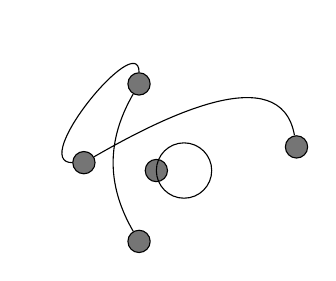
\begin{tikzpicture}
		\node[vertice](v1) at (1,0) {};
		\node[vertice](v2) at (1,2) {};
		\node[vertice](v3) at (3,1.2) {};
		\node[vertice](v4) at (0.3,1) {};
		\node[vertice](v5) at (1.22,0.9) {};
		\path[draw=black] 
			(v1) to[in=-120, out=120] (v2)
			(v3) to[in=30, out=100] (v4)
			(v2) to[out=90, in=180] (v4)
			(v5) arc[start angle=180, end angle=-180, radius=1em];
	\end{tikzpicture}
	\hfill
	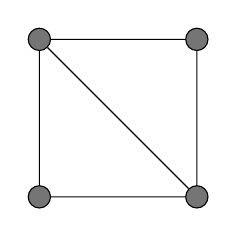
\begin{tikzpicture}[scale=1, transform shape]
		\node[vertice](v1) at (0,0) {};	
		\node[vertice](v2) at (2,0) {};	
		\node[vertice](v3) at (0,2) {};	
		\node[vertice](v4) at (2,2) {};	
		\path[draw=black]
			(v2)--(v4)--(v3)--(v1)--(v2)--(v3);
	\end{tikzpicture}
	\hfill
	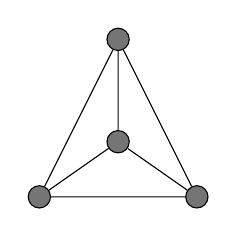
\begin{tikzpicture}
		\node[vertice](v1) at (0,0) {};
		\node[vertice](v2) at (2,0) {};
		\node[vertice](v3) at (1,2) {};
		\node[vertice](v4) at (1,0.7) {};
		\path[draw=black](v1)--(v2)--(v3)--(v1)--(v4)--(v2)--(v3)(v4)--(v3);
	\end{tikzpicture}
	\hfill~
	\caption{Minh họa một số đồ thị}
	\label{fig:minh-hoa-mot-so-do-thi}
\end{figure}


\begin{definition}[Đồ thị có hướng]
	Đồ thị $G=(V,E)$ là đồ thị có hướng $\iff \forall (u,v)\in E,\ (u,v)$ sắp thứ tự. Khi đó $u$ gọi là đỉnh ra, $v$ là đỉnh vào, cạnh $(u,v)$ gọi là một cung.
\end{definition}
\begin{figure}[htpb]
\begin{center}
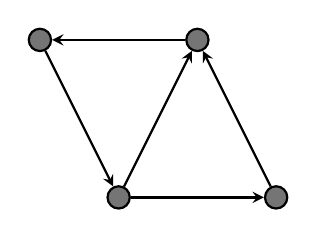
\begin{tikzpicture}[thick, ->, >=stealth, scale=1, transform shape]
	\node[vertice] (v1) at (0,2) {};
	\node[vertice] (v2) at (1,0) {};
	\node[vertice] (v3) at (3,0) {};
	\node[vertice] (v4) at (2,2) {};
	\draw (v1) -> (v2);
	\draw (v2) -> (v3);
	\draw (v3) -> (v4);
	\draw (v2) -> (v4);
	\draw (v4) -> (v1);
\end{tikzpicture}
\end{center}
\caption{Đồ thị có hướng}
\label{fig:do-thi-co-huong}
\end{figure}


\begin{definition}
	[Đồ thị có trọng số] Là đồ thị mà mỗi cạnh của nó được gắn với một trọng số.
\end{definition}
\begin{definition}
	[Đồ thị con] Đồ thị $H$ gọi là đồ thị con của $G \iff V(H) \subseteq V(G) \land E(H) \subseteq E(G)$. Kí hiệu:$H \subseteq G$. Nếu $H \subseteq G$ và $V(H) = V(G) = V$ thì ta gọi $H$ là đồ thị con mở rộng của $G$.
\end{definition}

\begin{definition}
	[Đồ thị đầy đủ/clique] Đồ thị $G$ là đồ thị đầy đủ (clique) $\iff$ mọi đỉnh của $G$ đều có cạnh nối giữa chúng. Đồ thị đầy đủ có $n$ đỉnh được kí hiệu là $K_n$. Đồ thị $\overline G$ được gọi là phủ của $G \iff$ $V(G)= V(\overline G)$ và $V(\overline G) = V(K_n) \setminus V(G)$
\end{definition}
\begin{figure}[htpb]
\begin{center}
\hfill
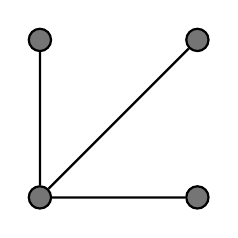
\begin{tikzpicture}[thick]
	\node[vertice](v1) at (0,0) {};
	\node[vertice](v2) at (2,0) {};
	\node[vertice](v3) at (2,2) {};
	\node[vertice](v4) at (0,2) {};
	\path[draw=black] (v1) -- (v2) (v1)--(v3) (v1)--(v4);
\end{tikzpicture}\hfill
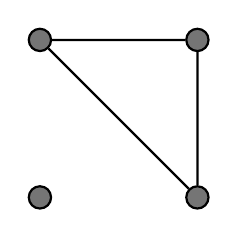
\begin{tikzpicture}[thick]
	\node[vertice](v1) at (0,0) {};
	\node[vertice](v2) at (2,0) {};
	\node[vertice](v3) at (2,2) {};
	\node[vertice](v4) at (0,2) {};
	\path[draw=black] (v2)--(v3)--(v4)--(v2);
\end{tikzpicture}\hfill~
\end{center}
\caption{Đồ thị $G$ và $\overline G$}
\label{fig:do-thi-g-va-g-ngang}
\end{figure}



\begin{definition}
	[Đồ thị hai phía] Đồ thị $G$ là đồ thị 2 phía $\iff V(G) = V_1 \cup V_2$ với $V_1, V_2$ là tập độc lập, $V_1 \cap V_2 = \varnothing$. Nếu $\forall u \in V_1, v \in V_2, v \textnormal{ kề } u$ thì $G$ gọi là đồ thị hai phía đầy đủ và được kí hiệu là $K_{m,n}$ (với $m = \abs{V_1}, n = \abs{V_2}$).	
\end{definition}
\begin{figure}[htpb]
\begin{center}
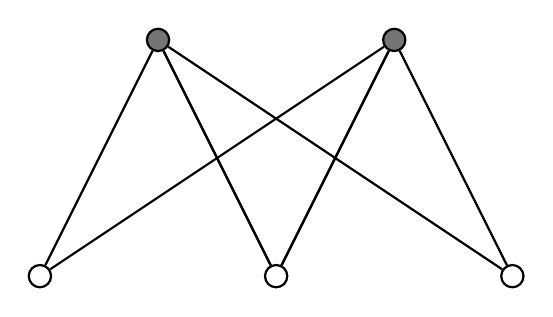
\begin{tikzpicture}[thick]
	\node[vertice, fill=white] (v1) at (0,0){};	
	\node[vertice, fill=white] (v2) at (3,0){};	
	\node[vertice, fill=white] (v3) at (6,0){};	
	\node[vertice] (v4) at (1.5,3){};	
	\node[vertice] (v5) at (4.5,3){};	
	\path[draw=black] (v1) -- (v4) -- (v2) -- (v5) -- (v3);
	\path[draw=black] (v1) -- (v5) -- (v2) -- (v4) -- (v3);
\end{tikzpicture}
\end{center}
\caption{Đồ thị hai phía đầy đủ $K_{2,3}$}
\label{fig:do-thi-hai-phia-day-du-k23}
\end{figure}



\begin{definition}
	[Tập độc lập] Tập độc lập trong đồ thị $G$ được định nghĩa bởi ${S = \{v \in V(G) \mid \textnormal{không có cặp đỉnh nào kề nhau} \}}$
\end{definition}

\begin{definition}
	[Đồ thị liên thông] Đồ thị $G$ gọi là liên thông $\iff \forall\ u,v \in V,\ \exists$ đường đi từ $u$ tới $v$. Ngược lại, nếu $\exists\ u,v \in V,\ \nexists$ đường đi từ $u$ tới $v$ thì $G$ là đồ thị \textbf{không} liên thông.
\end{definition}
\begin{figure}[htpb]
\begin{center}
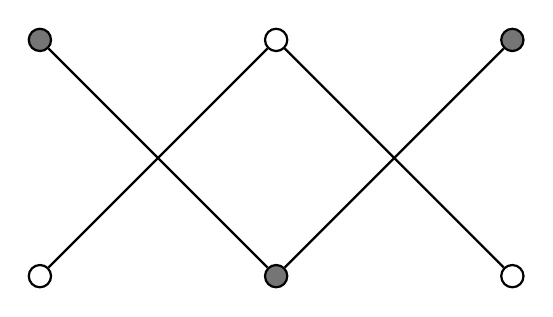
\begin{tikzpicture}[thick]
	\node[vertice, fill=white] (v1) at (0,0){};	
	\node[vertice, fill=white] (v3) at (6,0){};	
	\node[vertice, fill=white] (v5) at (3,3){};	
	\node[vertice] (v2) at (3,0){};	
	\node[vertice] (v4) at (0,3){};	
	\node[vertice] (v6) at (6,3){};	
	\path[draw=black] (v1) -- (v5) -- (v3);
	\path[draw=black] (v4) -- (v2) -- (v6);
\end{tikzpicture}
\end{center}
\caption{Đồ thị không liên thông}
\label{fig:do-thi-khong-lien-thong}
\end{figure}




\section{Đường đi và chu trình}
\begin{definition}[đường đi]
	\label{def:duong-di}
	Một \textbf{đường đi} (kí hiệu W) có độ dài $k$ là một dãy các \textbf{đỉnh và cạnh} $v_0, e_1, v_1, e_2,\cdots,e_k,v_k$ với $e_i = (v_{i-1},v_i)$. Độ dài của một đường đi kí hiệu là $l(W)$. Đỉnh $v_0$ gọi là đỉnh đầu và $v_k$ gọi là đỉnh cuối. Nếu không có cạnh nào lặp lại, đường đi gọi là đơn. Nếu không có đỉnh nào lặp lại, đường đi gọi là sơ cấp.
\end{definition}
\begin{definition}[chu trình]
	\label{def:chu-trinh}
	 Một chu trình là một đường đi đơn mà có đỉnh đầu và đỉnh cuối trùng nhau. Nếu chỉ có đỉnh đầu và đỉnh cuối trùng nhau thì chu trình gọi là sơ cấp.
\end{definition}
Có thể thấy chu trình với độ dài 1 là một khuyên.
\begin{proposition}
	Đồ thị $G$ là liên thông $\iff ({\exists uv \in E})({ u\in V_1})({v \in V_2})$ với mọi $V_1,\,V_2 \ne \varnothing$ mà $V = V_1\cup V_2,\, V_1 \cap V_2 = \varnothing$ ($V_1,\,V_2$ là phân hoạch không rỗng của $V$)
	\begin{proof}
		Giả sử $G$ liên thông. Khi đó tồn tại một đường đi sơ cấp từ $u$ tới $v$, trên đường đi đó, sau đỉnh cuối cùng của $V_1$ mà nó đi qua là cạnh nối giữa $V_1$ và $V_2$. Giả sử $G$ không liên không. Chứng minh được chiều xuôi.\\
		Gọi $H$ là một thành phần liên thông của $G$, chọn $V_1 = V(H)$. Khi đó không có cạnh nào của $G$ có một đầu mút thuộc $V_1$ và đầu mút còn lại thuộc $V_2$. Bằng cách đảo vế chứng minh được chiều ngược.
	\end{proof}
\end{proposition}

\begin{theorem}
Một cạnh của $G$ là cạnh cắt $\iff$ cạnh đó không thuộc chu trình nào.	
\begin{proof}
	Gọi $e=(uv)$ là một cạnh trong thành phần liên thông $H$ của $G$. Nếu đồ thị thu được từ $H$ bỏ đi $e$ (kí hiệu $H-e$) vẫn liên thông, thì tồn tại một đường đi sơ cấp từ $u$ tới $v$. Có thể thấy đường đi này nếu gắn thêm cạnh $e$ sẽ tạo thành một chu trình . Vậy nếu $e$ không phải cạnh cắt thì sẽ thuộc một chu trình . \\
	Gọi thành phần liên thông của $G$ chứa $e$ là $H$, $e = (x,y)$ nằm trong chu trình $C$. Lấy bất kì $u,v \in H$. Gọi $P$ là một đường đi bất kì từ $u$ tới $v$. Nếu $P$ không chứa $e$ thì ta có đpcm. Nếu $P$ chứa $e$ thì $P$ đi qua $x$ và $y$. Vì $e$ nằm trong chu trình $C$ nên dù bỏ cạnh $e$ thì vẫn tồn tại một đường đi $P'$ từ $x$ tới $y$, chỉ cần thay $x,e,y$ trong $P$ bằng $P'$ ta lại có một đường đi từ $u \to x \to y \to v$. Do đó nếu bỏ cạnh $e$ thì vẫn tồn tại đường đi từ $u$ tới $v$, suy ra $H-e$ liên thông. Vậy nếu cạnh $e$ thuộc một chu trình thì $e$ không phải cạnh cắt.
\end{proof}
\end{theorem}

\begin{proposition}
	Cho đồ thị $G = (V,E)$, $V=\{v_1, v_2,\ldots,v_n\}$ với $n \ge 3$. Nếu có ít nhất 2 trong các đồ thị con $G-v_1,G-v_2,\ldots,G-v_n$ ($G$ xóa đi đỉnh $v_i$) liên thông thì $G$ liên thông.
	\begin{proof}
		Giả sử $G$ không liên thông, $H_i,\, i = \overline{1,k}$ là các thành phần liên thông của $G$. Nếu xóa một đỉnh khỏi $H_i$ thì không làm thay đổi số thành phần liên thông, trừ khi $H_i = K_1$ (giảm đi còn $k-1$ thành phần liên thông). Nếu 2 trong số $G-v_1,G-v_2,\ldots,G-v_n$ liên thông thì $k = 2$ và $H_1 = H_2 = K_1$, mâu thuẫn với $n \ge 3$.
	\end{proof}
\end{proposition}

\begin{corolarry} Mọi đồ thị $G$ mà chứa ít nhất một cạnh thì có ít nhất hai đỉnh không phải là đỉnh cắt\end{corolarry}
\begin{theorem}
Một đồ thị là một đồ thị hai phía $\iff$ nó không chứa chu trình độ dài lẻ.	
\begin{proof}
	Giả sử $G$ là một đồ thị hai phía, khi đó mọi đường đi trên $G$ đều chuyển qua chuyển lại giữa các đỉnh thuộc $V_1$ và $V_2$. Vì vậy, nếu muốn quay lại điểm bắt đầu thì đường đi buộc phải có độ dài chẵn.\\
	Giả sử $G$ không có chu trình độ dài chẵn. $G$ liên thông. Chọn cố định điểm $u$ thuộc $V(G)$. Với mọi điểm $v \in V(G)$, mọi đường đi từ $u$ tới $v$ đều phải có độ dài cùng chẵn hoặc cùng lẻ, nếu không sẽ tạo ra một chu trình độ dài lẻ (mâu thuẫn). Ta phân hoạch $V(G)$ thành 2 tập $V_1 = \{v\mid$ đường đi từ $u$ tới $v$ độ dài lẻ $\}$ và $V_2 = \{v\mid$ đường đi từ $u$ tới $v$ độ dài chẵn $\}$. Thấy được $V_1$ là một tập độc lập vì một cạnh nối giữa hai đỉnh của $V_1$ sẽ tạo ra một chu trình độ dài lẻ. Ta có điều tương tự với $V_2$. Do đó $G$ là một đồ thị hai phía.
\end{proof}
\end{theorem}




\section{Biểu diễn đồ thị bằng ma trận}
Đồ thị $G$ có thể được biểu diễn bằng một ma trận $A(G) = [a_{ij}]$ với $a_{ij}$ là số cạnh nối nữa $v_i$ và $v_j$. Nếu $G$ là đồ thị có hướng, $a_{ij}$ sẽ là số cung đi từ $v_i$ tới $v_j$.

Nếu cạnh $e$ có đầu mút là đỉnh $v$ thì $e$ gọi là cạnh kề của $v$. Đồ thị G cũng có thể biểu diễn bằng ma trận $M = [m_{ij}]$, trong đó $m_{ij} = 1$ nếu đỉnh $v_i$ có cạnh kề $e_j$. Trong trường hợp $G$ là đồ thị có hướng, $m_{ij} = 1$ nếu $v_i$ là đỉnh ra  và $-1$ nếu $v_i$ là đỉnh vào của $e_j$. Nếu không rơi vào những trường hợp trên thì $m_{ij} = 0$.


\begin{figure}[h]
	\begin{center}
		\begin{minipage}[c]{0.3\textwidth}
			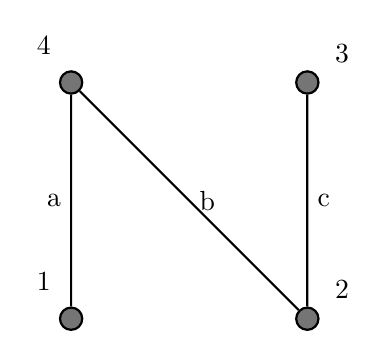
\begin{tikzpicture}[thick]
				\node[vertice, label={[label distance=1mm]120:1}] (v1) at (0,0) {};
				\node[vertice, label={[label distance=1mm]30:2}] (v2) at (3,0) {};
				\node[vertice, label={[label distance=1mm]30:3}] (v3) at (3,3) {};
				\node[vertice, label={[label distance=1mm]120:4}] (v4) at (0,3) {};
				\path[draw=black] (v1) 
					--node[anchor=east]{a} (v4) 
					--node[anchor=west]{b} (v2) 
					--node[anchor=west]{c} (v3);
			\end{tikzpicture}
		\end{minipage}
		\begin{minipage}[c]{0.3\textwidth}
			\begin{align*}
				\left(
					\begin{array}{c|cccc}
						&1&2&3&4\\\hline
						1&0&0&0&1\\
						2&0&0&1&1\\
						3&0&1&0&0\\
						4&1&1&0&0
					\end{array}
				\right)
			\end{align*}
		\end{minipage}
		\begin{minipage}[c]{0.3\textwidth}
			\begin{align*}
				\left(
					\begin{array}{c|ccc}
						 &a&b&c\\\hline
						1&1&0&0\\
						2&0&1&1\\
						3&0&0&1\\
						4&1&1&0
					\end{array}
				\right)
			\end{align*}
		\end{minipage}\par
		\begin{minipage}{0.3\textwidth}\begin{center}$G$\end{center}\end{minipage}
		\begin{minipage}{0.3\textwidth}\begin{center}$A(G)$\end{center}\end{minipage}
		\begin{minipage}{0.3\textwidth}\begin{center}$M(G)$\end{center}\end{minipage}
	\end{center}
	\caption{Biểu diễn đồ thị $G$}
	\label{fig:bieu-dien-do-thi-g}
\end{figure}

\begin{figure}[ht]
	\begin{center}
		\begin{minipage}[c]{0.3\textwidth}
			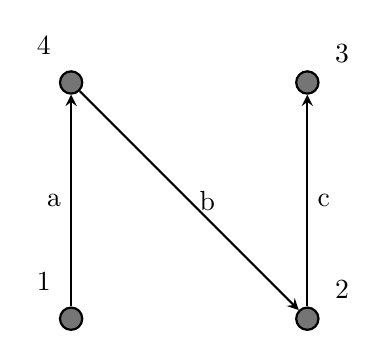
\begin{tikzpicture}[->, >=stealth, thick]
				\node[vertice, label={[label distance=1mm]120:1}] (v1) at (0,0) {};
				\node[vertice, label={[label distance=1mm]30:2}] (v2) at (3,0) {};
				\node[vertice, label={[label distance=1mm]30:3}] (v3) at (3,3) {};
				\node[vertice, label={[label distance=1mm]120:4}] (v4) at (0,3) {};
				\draw (v1)--node[anchor=east]{a} (v4);
				\draw (v4)--node[anchor=west]{b} (v2);
				\draw (v2)--node[anchor=west]{c} (v3);
			\end{tikzpicture}
		\end{minipage}
		\begin{minipage}[c]{0.3\textwidth}
			\begin{align*}
				\left(
					\begin{array}{c|cccc}
						&1&2&3&4\\\hline
						1&0&0&0&1\\
						2&0&0&1&0\\
						3&0&0&0&0\\
						4&0&1&0&0
					\end{array}
				\right)
			\end{align*}
		\end{minipage}
		\begin{minipage}[c]{0.3\textwidth}
			\begin{align*}
				\left(
					\begin{array}{c|rrr}
						 &a&b&c\\\hline
						1&+1& 0& 0\\
						2& 0&-1&+1\\
						3& 0& 0&-1\\
						4&-1&+1& 0
					\end{array}
				\right)
			\end{align*}
		\end{minipage}\par
		\begin{minipage}{0.3\textwidth}\begin{center}$G$\end{center}\end{minipage}
		\begin{minipage}{0.3\textwidth}\begin{center}$A(G)$\end{center}\end{minipage}
		\begin{minipage}{0.3\textwidth}\begin{center}$M(G)$\end{center}\end{minipage}
	\end{center}
	\caption{Biểu diễn đồ thị $G$ (có hướng)}
	\label{fig:bieu-dien-do-thi-g-co-huong}
\end{figure}



Một đồ thị có thể có nhiều ma trận $A(G)$ hoặc $M(G)$ khác nhau, tùy vào cách đánh số cạnh/đỉnh. Sau đây là một số tính chất:
\begin{itemize}
	\item Nếu $A(G)$ là ma trận đối xứng thì đồ thị $G$ vô hướng. 
	\item Nếu $A(G)$ đối xứng, $a_{ij} \in \{0,1\}$ và $a_{ii} = 0$ thì $G$ là đồ thị đơn giản.
\end{itemize}

\begin{definition}
	[Đẳng cấu]
	Một đẳng cấu giữa $G$ và $H$ là ánh xạ ${f: V(G) \to V(H)}$ sao cho $\forall\ u,v \in V(G)$ thì $f(u)f(v) \in V(H)$. Nếu tìm được một đẳng cấu từ $G$ tới $H$ và ngược lại, ta nói $G$ và $H$ đẳng cấu nhau.
\end{definition}

Đồ thị $G$ và $H$ được gọi là đẳng cấu $\iff$ có thể áp dụng biến đổi trên hàng của $A(G)$ \textbf{và} áp dụng biến đổi tương tự trên cột của $A(G)$ để thu được $A(H)$.

\begin{figure}[h]
	\begin{center}
		\begin{minipage}[c]{0.4\textwidth}
			\begin{center}
				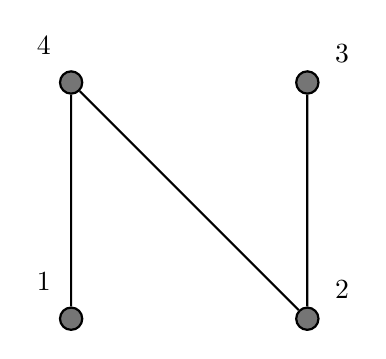
\begin{tikzpicture}[thick]
					\node[vertice, label={[label distance=1mm]120:1}] (v1) at (0,0) {};
					\node[vertice, label={[label distance=1mm]30:2}] (v2) at (3,0) {};
					\node[vertice, label={[label distance=1mm]30:3}] (v3) at (3,3) {};
					\node[vertice, label={[label distance=1mm]120:4}] (v4) at (0,3) {};
					\path[draw=black] (v1) -- (v4) -- (v2) -- (v3);
				\end{tikzpicture}
			\end{center}
		\end{minipage}
		\begin{minipage}[c]{0.4\textwidth}
			\begin{center}
				\begin{align*}
					\left(
						\begin{array}{c|cccc}
						&1&2&3&4\\\hline
							1&0&0&0&1\\
							2&0&0&1&1\\
							3&0&1&0&0\\
							4&1&1&0&0
						\end{array}
					\right)
				\end{align*}
			\end{center}
		\end{minipage}
		\begin{minipage}{0.4\textwidth}\begin{center}$G$\end{center}\end{minipage}
		\begin{minipage}{0.4\textwidth}\begin{center}$A(G)$\end{center}\end{minipage}
		\begin{minipage}[c]{0.4\textwidth}
			\begin{center}
				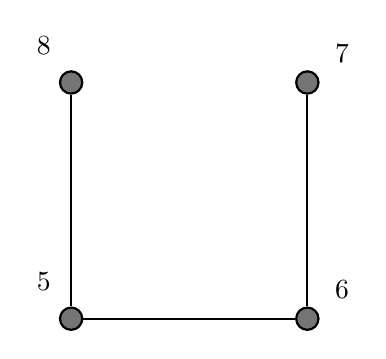
\begin{tikzpicture}[thick]
					\node[vertice, label={[label distance=1mm]120:5}] (v5) at (0,0) {};
					\node[vertice, label={[label distance=1mm] 30:7}] (v7) at (3,3) {};
					\node[vertice, label={[label distance=1mm] 30:6}] (v6) at (3,0) {};
					\node[vertice, label={[label distance=1mm]120:8}] (v8) at (0,3) {};
					\path[draw=black] (v8) -- (v5) -- (v6) -- (v7);
				\end{tikzpicture}
			\end{center}
		\end{minipage}
		\begin{minipage}[c]{0.4\textwidth}
			\begin{center}
				\begin{align*}
					\left(
						\begin{array}{c|cccc}
							 &5&6&7&8\\\hline
							5&0&1&0&1\\
							6&1&0&1&0\\
							7&0&1&0&0\\
							8&1&0&0&0
						\end{array}
					\right)
				\end{align*}
			\end{center}
		\end{minipage}
		\begin{minipage}{0.4\textwidth}\begin{center}$H$\end{center}\end{minipage}
		\begin{minipage}{0.4\textwidth}\begin{center}$A(H)$\end{center}\end{minipage}
	\end{center}
	\caption{Đẳng cấu $H$ và $G$}
	\label{fig:dong-cau-h-va-g}
\end{figure}



Trong hình \ref{fig:dong-cau-h-va-g}, đẳng cấu $f$ được xác định: $f(1) = 8$; $f(2) = 6$; $f(3) = 7$; $f(4) = 5$. Từ ma trận $A(G)$ có thể thu được $A(H)$ bằng cách đổi chỗ hai hàng $1,4$ và rồi đổi chỗ hai cột tương ứng.

Đẳng cấu đồ thị là quan hệ tương đương, do đó ta có các lớp tương đương. Một lớp tương đương đẳng cấu đồ thị được biểu diễn bằng một đồ thị \textit{không được gán nhãn}. Dễ thấy đồ thị $G$ và $H$ trong hình \ref{fig:dong-cau-h-va-g} cùng thuộc một lớp tương đương. Ta kí hiệu $G = H$ thay vì $G \cong H$. Tương tự, khi nói $H$ là đồ thị con của $G$, điều này có nghĩa $H$ đẳng cấu với một đồ thị con của $G$, hay $G$ chứa một bản sao của $H$. 

Đẳng cấu bảo toàn quan hệ "kề nhau" giữa các cạnh, do đó nếu muốn chứng minh hai đồ thị không đẳng cấu, ta chỉ cần chỉ ra một đặc tính nào đó liên quan tới đỉnh mà chúng khác nhau (\textit{bậc của các đỉnh, kích cỡ của clique lớn nhất hoặc chu kì nhỏ nhất\ldots}).

Hai đồ thị $G$ và $H$ đẳng cấu $\iff \overline{G} \textnormal{ đẳng cấu } \overline{H}$.

\begin{definition}[tự đẳng cấu]
	Một tự đẳng cấu là một đẳng cấu của đồ thị $G$ với chính nó. $G$ gọi là chuyển tiếp đỉnh $\iff ({\forall\ u,v \in V})\ ({\exists f: f(u) = v})$. Tương tự, $G$ gọi là chuyển tiếp cạnh $\iff ({\forall\ e_1,e_2 \in E})\ ({\exists f: f(e_1) = e_2})$.
\end{definition}




\section{Đẳng cấu đồ thị}
\begin{definition}
	[Đẳng cấu]
	Một đẳng cấu giữa $G$ và $H$ là ánh xạ ${f: V(G) \to V(H)}$ sao cho $\forall\ u,v \in V(G)$ thì $f(u)f(v) \in V(H)$. Nếu tìm được một đẳng cấu từ $G$ tới $H$ và ngược lại, ta nói $G$ và $H$ đẳng cấu nhau.
\end{definition}

Đồ thị $G$ và $H$ được gọi là đẳng cấu $\iff$ có thể áp dụng biến đổi trên hàng của $A(G)$ \textbf{và} áp dụng biến đổi tương tự trên cột của $A(G)$ để thu được $A(H)$.

\begin{figure}[h]
	\begin{center}
		\begin{minipage}[c]{0.4\textwidth}
			\begin{center}
				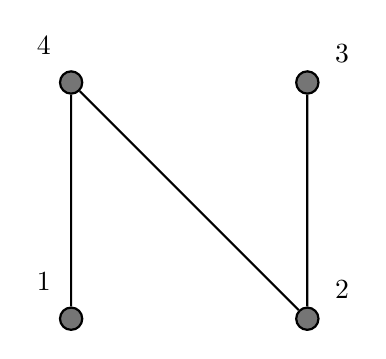
\begin{tikzpicture}[thick]
					\node[vertice, label={[label distance=1mm]120:1}] (v1) at (0,0) {};
					\node[vertice, label={[label distance=1mm]30:2}] (v2) at (3,0) {};
					\node[vertice, label={[label distance=1mm]30:3}] (v3) at (3,3) {};
					\node[vertice, label={[label distance=1mm]120:4}] (v4) at (0,3) {};
					\path[draw=black] (v1) -- (v4) -- (v2) -- (v3);
				\end{tikzpicture}
			\end{center}
		\end{minipage}
		\begin{minipage}[c]{0.4\textwidth}
			\begin{center}
				\begin{align*}
					\left(
						\begin{array}{c|cccc}
						&1&2&3&4\\\hline
							1&0&0&0&1\\
							2&0&0&1&1\\
							3&0&1&0&0\\
							4&1&1&0&0
						\end{array}
					\right)
				\end{align*}
			\end{center}
		\end{minipage}
		\begin{minipage}{0.4\textwidth}\begin{center}$G$\end{center}\end{minipage}
		\begin{minipage}{0.4\textwidth}\begin{center}$A(G)$\end{center}\end{minipage}
		\begin{minipage}[c]{0.4\textwidth}
			\begin{center}
				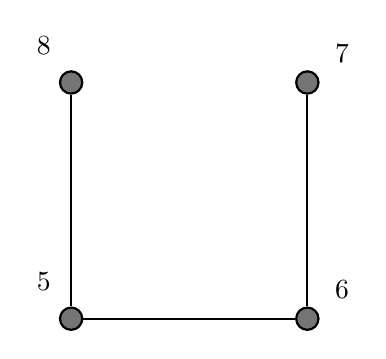
\begin{tikzpicture}[thick]
					\node[vertice, label={[label distance=1mm]120:5}] (v5) at (0,0) {};
					\node[vertice, label={[label distance=1mm] 30:7}] (v7) at (3,3) {};
					\node[vertice, label={[label distance=1mm] 30:6}] (v6) at (3,0) {};
					\node[vertice, label={[label distance=1mm]120:8}] (v8) at (0,3) {};
					\path[draw=black] (v8) -- (v5) -- (v6) -- (v7);
				\end{tikzpicture}
			\end{center}
		\end{minipage}
		\begin{minipage}[c]{0.4\textwidth}
			\begin{center}
				\begin{align*}
					\left(
						\begin{array}{c|cccc}
							 &5&6&7&8\\\hline
							5&0&1&0&1\\
							6&1&0&1&0\\
							7&0&1&0&0\\
							8&1&0&0&0
						\end{array}
					\right)
				\end{align*}
			\end{center}
		\end{minipage}
		\begin{minipage}{0.4\textwidth}\begin{center}$H$\end{center}\end{minipage}
		\begin{minipage}{0.4\textwidth}\begin{center}$A(H)$\end{center}\end{minipage}
	\end{center}
	\caption{Đẳng cấu $H$ và $G$}
	\label{fig:dong-cau-h-va-g}
\end{figure}



Trong hình \ref{fig:dong-cau-h-va-g}, đẳng cấu $f$ được xác định: $f(1) = 8$; $f(2) = 6$; $f(3) = 7$; $f(4) = 5$. Từ ma trận $A(G)$ có thể thu được $A(H)$ bằng cách đổi chỗ hai hàng $1,4$ và rồi đổi chỗ hai cột tương ứng.

Đẳng cấu đồ thị là quan hệ tương đương, do đó ta có các lớp tương đương. Một lớp tương đương đẳng cấu đồ thị được biểu diễn bằng một đồ thị \textit{không được gán nhãn}. Dễ thấy đồ thị $G$ và $H$ trong hình \ref{fig:dong-cau-h-va-g} cùng thuộc một lớp tương đương. Ta kí hiệu $G = H$ thay vì $G \cong H$. Tương tự, khi nói $H$ là đồ thị con của $G$, điều này có nghĩa $H$ đẳng cấu với một đồ thị con của $G$, hay $G$ chứa một bản sao của $H$. 

Đẳng cấu bảo toàn quan hệ "kề nhau" giữa các cạnh, do đó nếu muốn chứng minh hai đồ thị không đẳng cấu, ta chỉ cần chỉ ra một đặc tính nào đó liên quan tới đỉnh mà chúng khác nhau (\textit{bậc của các đỉnh, kích cỡ của clique lớn nhất hoặc chu kì nhỏ nhất\ldots}).

Hai đồ thị $G$ và $H$ đẳng cấu $\iff \overline{G} \textnormal{ đẳng cấu } \overline{H}$.

\begin{definition}[tự đẳng cấu]
	Một tự đẳng cấu là một đẳng cấu của đồ thị $G$ với chính nó. $G$ gọi là chuyển tiếp đỉnh $\iff ({\forall\ u,v \in V})\ ({\exists f: f(u) = v})$. Tương tự, $G$ gọi là chuyển tiếp cạnh $\iff ({\forall\ e_1,e_2 \in E})\ ({\exists f: f(e_1) = e_2})$.
\end{definition}





\section{Một số phép toán trên đồ thị}
\label{sec:mot_so_phep_toan_tren_do_thi}
\begin{definition}
	[Phép hợp] Đồ thị $G = (V,E)$ gọi là hợp của đồ thị $G_1$ và $G_2 \iff V(G) = V(G_1) \cup V(G_2)$ và $E(G) = E(G_1) \cup E(G_2)$. Ký hiệu $G = G_1\cup G_2$. Nếu $V_1 \cap V_2 = \varnothing$ ta viết $G = G_1 + G_2$. Ta cũng định nghĩa $mG$ là hợp $m$ lần các bản sao của $G$.
\end{definition}
\begin{definition}
	[Phép hội] Đồ thị $G = G_1 \lor G_2 \iff$ $V(G) = V(G_1 + G_2) \land E(G) = E(G_1 +G_2) \cup \left\{e=uv\mid u \in V_1, v \in V_2\right\}$ (Đồ thị $G_1 +G_2$ thêm vào những cạnh nối giữa các đỉnh của chúng).
\end{definition}
\begin{figure}[htpb]
\begin{center}
	\begin{minipage}{0.45\textwidth}
		\begin{center}
		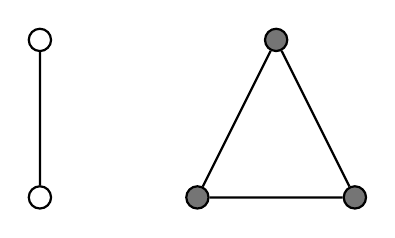
\begin{tikzpicture}[thick]
			\node[vertice, fill=white] (p1) at (0,0) {};
			\node[vertice, fill=white] (p2) at (0,2) {};
			\node[vertice] (c1) at (2,0) {};
			\node[vertice] (c2) at (4,0) {};
			\node[vertice] (c3) at (3,2) {};
			\path[draw=black] (p1)--(p2)(c1)--(c2)--(c3)--(c1);
		\end{tikzpicture}
		\end{center}
	\end{minipage}
	\begin{minipage}{0.45\textwidth}
		\begin{center}
		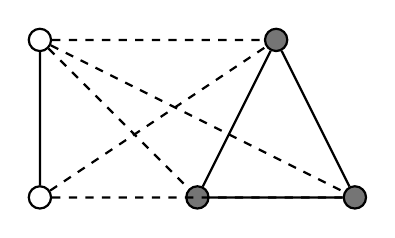
\begin{tikzpicture}[thick]
			\node[vertice, fill=white] (p1) at (0,0) {};
			\node[vertice, fill=white] (p2) at (0,2) {};
			\node[vertice] (c1) at (2,0) {};
			\node[vertice] (c2) at (4,0) {};
			\node[vertice] (c3) at (3,2) {};
			\path[draw=black] 
				(p2)[dashed]--(c1)(p2)[dashed]--(c2)(p2)[dashed]--(c3)
				(p1)[dashed]--(c1)(p1)[dashed]--(c2)(p1)[dashed]--(c3);
			\path[draw=black]
				(p1)--(p2)(c1)--(c2)--(c3)--(c1);
		\end{tikzpicture}
		\end{center}
	\end{minipage}
\end{center}
\caption{hợp/hội đồ thị $p_2$ và $c_3$}
\label{fig:hop_hoi_do_thi_p2_c3}
\end{figure}



\begin{definition}
	[tích descartes] Đồ thị $G = G_1 \times G_2$ là đồ thị mà $V(G) = \left\{(v_i,u_i)\right\}$ $v_i \in V_1,\, u_i \in V_2$. Có $k$ cạnh nối $(v_i,u_i)$ với $(v_j,u_j) \iff {(v_i = v_j)} \land (u_i $ nối với $u_j$ $k$ lần  trong $G_2)$ hoặc ${(u_i = u_j)} \land (v_i $ nối với $v_j$ $k$ lần  trong $G_1)$.
\end{definition}

\begin{figure}[htpb]
\begin{center}
	\begin{minipage}{0.4\textwidth}
		\begin{center}
		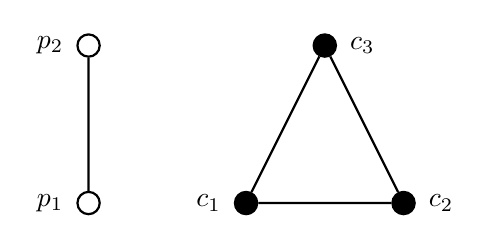
\begin{tikzpicture}[thick]
			\node[label={[label distance=1pt]180:$p_1$}, vertice, fill=white] (p1) at (0,0) {};
			\node[label={[label distance=1pt]180:$p_2$}, vertice, fill=white] (p2) at (0,2) {};
			\node[label={[label distance=1pt]180:$c_1$}, vertice, fill=black] (c1) at (2,0) {};
			\node[label={[label distance=1pt]000:$c_2$}, vertice, fill=black] (c2) at (4,0) {};
			\node[label={[label distance=1pt]000:$c_3$}, vertice, fill=black] (c3) at (3,2) {};
			\path[draw=black] (p1)--(p2)(c1)--(c2)--(c3)--(c1);
		\end{tikzpicture}
		\end{center}
	\end{minipage}
	\begin{minipage}[m]{0.05\textwidth}
		$\implies$
	\end{minipage}
	\begin{minipage}{0.45\textwidth}
		\begin{center}
		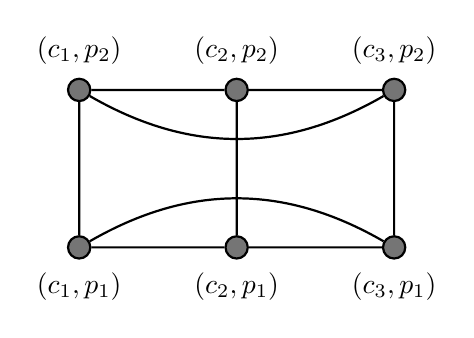
\begin{tikzpicture}[thick]
			\node[label={[label distance=1pt]270:$(c_1,p_1)$}, vertice] (c1p1) at (0,0) {};
			\node[label={[label distance=1pt]090:$(c_1,p_2)$}, vertice] (c1p2) at (0,2) {};
			\node[label={[label distance=1pt]270:$(c_2,p_1)$}, vertice] (c2p1) at (2,0) {};
			\node[label={[label distance=1pt]090:$(c_2,p_2)$}, vertice] (c2p2) at (2,2) {};
			\node[label={[label distance=1pt]270:$(c_3,p_1)$}, vertice] (c3p1) at (4,0) {};
			\node[label={[label distance=1pt]090:$(c_3,p_2)$}, vertice] (c3p2) at (4,2) {};
			\path[draw=black] 
				(c1p1)--(c2p1)--(c3p1) to[in =  30,out=150] (c1p1)
				(c1p2)--(c2p2)--(c3p2) to[out=-150,in =-30] (c1p2)
				(c3p1)--(c3p2)
				(c2p1)--(c2p2)
				(c1p1)--(c1p2);
		\end{tikzpicture}
		\end{center}
	\end{minipage}
\end{center}
\caption{Tích descartes $P_2 \times C_3$}
\label{fig:tich_descartes_p2_x_c3}
\end{figure}
\begin{definition}
	[tích tensor] Tích tensor của $G$, kí hiệu $G_1 \cdot G_2$, là một đồ thị với $V(G) = V(G_1) \times V(G_2)$. Với $u_i \in V_1$, $v_i \in V_2$, có $k$ cạnh nối giữa $(u_i,v_i)$ và $(u_j,v_j) \iff ($có $m$ cạnh nối $u_i$ với $u_j$, $n$ cạnh nối $v_i$ với $v_j) \land (k = m\cdot n)$.
\end{definition}

\begin{figure}[htpb]
\begin{center}
	\begin{minipage}{0.4\textwidth}
		\begin{center}
		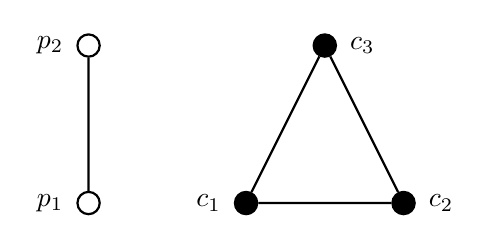
\begin{tikzpicture}[thick]
			\node[label={[label distance=1pt]180:$p_1$}, vertice, fill=white] (p1) at (0,0) {};
			\node[label={[label distance=1pt]180:$p_2$}, vertice, fill=white] (p2) at (0,2) {};
			\node[label={[label distance=1pt]180:$c_1$}, vertice, fill=black] (c1) at (2,0) {};
			\node[label={[label distance=1pt]000:$c_2$}, vertice, fill=black] (c2) at (4,0) {};
			\node[label={[label distance=1pt]000:$c_3$}, vertice, fill=black] (c3) at (3,2) {};
			\path[draw=black] (p1)--(p2)(c1)--(c2)--(c3)--(c1);
		\end{tikzpicture}
		\end{center}
	\end{minipage}
	\begin{minipage}[m]{0.05\textwidth}
		$\implies$
	\end{minipage}
	\begin{minipage}{0.45\textwidth}
		\begin{center}
		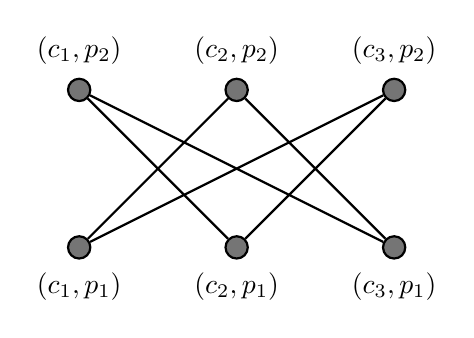
\begin{tikzpicture}[thick]
			\node[label={[label distance=1pt]270:$(c_1,p_1)$}, vertice] (c1p1) at (0,0) {};
			\node[label={[label distance=1pt]090:$(c_1,p_2)$}, vertice] (c1p2) at (0,2) {};
			\node[label={[label distance=1pt]270:$(c_2,p_1)$}, vertice] (c2p1) at (2,0) {};
			\node[label={[label distance=1pt]090:$(c_2,p_2)$}, vertice] (c2p2) at (2,2) {};
			\node[label={[label distance=1pt]270:$(c_3,p_1)$}, vertice] (c3p1) at (4,0) {};
			\node[label={[label distance=1pt]090:$(c_3,p_2)$}, vertice] (c3p2) at (4,2) {};
			\path[draw=black]
				(c1p2)--(c2p1)--(c3p2)--(c1p1)--(c2p2)--(c3p1)--(c1p2);
		\end{tikzpicture}
		\end{center}
	\end{minipage}
\end{center}
\caption{Tích tensor $P_2 \cdot C_3$}
\label{fig:tich_tensor_p2_c3}
\end{figure}

\begin{definition}
	[tích strong] Tích strong của $G$, kí hiệu $G = G_1 \circledast G_2$, được định nghĩa $G_1 \circledast G_2 = (G_1 \times G_2) \cup (G_1 \cdot G_2)$.
\end{definition}

\begin{figure}[htpb]
\begin{center}
	\begin{minipage}{0.4\textwidth}
		\begin{center}
		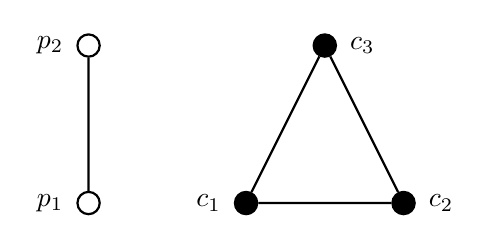
\begin{tikzpicture}[thick]
			\node[label={[label distance=1pt]180:$p_1$}, vertice, fill=white] (p1) at (0,0) {};
			\node[label={[label distance=1pt]180:$p_2$}, vertice, fill=white] (p2) at (0,2) {};
			\node[label={[label distance=1pt]180:$c_1$}, vertice, fill=black] (c1) at (2,0) {};
			\node[label={[label distance=1pt]000:$c_2$}, vertice, fill=black] (c2) at (4,0) {};
			\node[label={[label distance=1pt]000:$c_3$}, vertice, fill=black] (c3) at (3,2) {};
			\path[draw=black] (p1)--(p2)(c1)--(c2)--(c3)--(c1);
		\end{tikzpicture}
		\end{center}
	\end{minipage}
	\begin{minipage}[m]{0.05\textwidth}
		$\implies$
	\end{minipage}
	\begin{minipage}{0.45\textwidth}
		\begin{center}
		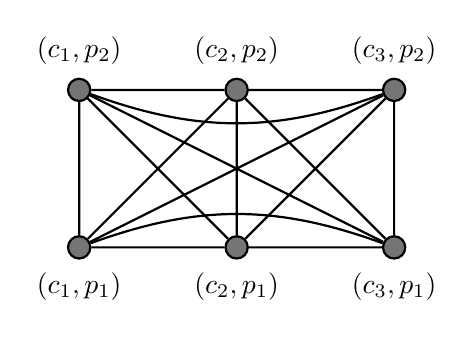
\begin{tikzpicture}[thick]
			\node[label={[label distance=1pt]270:$(c_1,p_1)$}, vertice] (c1p1) at (0,0) {};
			\node[label={[label distance=1pt]090:$(c_1,p_2)$}, vertice] (c1p2) at (0,2) {};
			\node[label={[label distance=1pt]270:$(c_2,p_1)$}, vertice] (c2p1) at (2,0) {};
			\node[label={[label distance=1pt]090:$(c_2,p_2)$}, vertice] (c2p2) at (2,2) {};
			\node[label={[label distance=1pt]270:$(c_3,p_1)$}, vertice] (c3p1) at (4,0) {};
			\node[label={[label distance=1pt]090:$(c_3,p_2)$}, vertice] (c3p2) at (4,2) {};
			\path[draw=black]
				(c1p2)--(c2p1)--(c3p2)--(c1p1)--(c2p2)--(c3p1)--(c1p2);
			\path[draw=black] 
				(c1p1)--(c2p1)--(c3p1) to[in =  20,out=160] (c1p1)
				(c1p2)--(c2p2)--(c3p2) to[out=-160,in =-20] (c1p2)
				(c3p1)--(c3p2)
				(c2p1)--(c2p2)
				(c1p1)--(c1p2);
		\end{tikzpicture}
		\end{center}
	\end{minipage}
\end{center}
\caption{Tích strong $P_2 \circledast C_3$}
\label{fig:tich_strong_p2_c3}
\end{figure}
%
%



\chapter{Các tính chất}
\label{sec:mot_so_dinh_ly_menh_de}
\section{Một số định lý}
\begin{theorem}
	\label{theo:tong_bac_cua_dinh} Cho một đồ thị $G$, tổng bậc của các đỉnh trong $G$ bằng 2 lần số cạnh của $G$.
	\begin{equation*}
		\sum_{\mathclap{\forall v \in V(G)}}d(v) = 2\abs{E(G)}
	\end{equation*}
	\begin{proof}
		Với mỗi $e \in E(G)$, $e$ có hai đầu mút, làm tăng bậc của $2$ đỉnh đầu mút của nó lên 1 và do đó tăng tổng số bậc của đồ thị lên 2.
	\end{proof}
\end{theorem}
\begin{corollary}
	\label{coro:number_of_odd_degree_vertices_is_even}
Số đỉnh bậc lẻ trong một đồ thị luôn là số chẵn. Không có đồ thị chính quy nào có bậc lẻ.
\end{corollary}
\begin{corollary}
	Đồ thị $k$ -- chính quy với $n$ đỉnh có $nk/2$ cạnh.
\end{corollary}

\begin{theorem}
	\label{theo:sub_bigraph}
	Cho đồ thị $G$ không có khuyên. Khi đó $G$ có một đồ thị con là đồ thị hai phía với ít nhất $\abs{E(G)}/2$ cạnh
	\begin{proof}
		Phân hoạch tập đỉnh của $G$ thành hai tập $V_1$ và $V_2$. Lấy các cạnh $e=uv$ sao cho $u \in V_1$ và $v\in V_2$ đưa vào tập $E(H)$. Khi đó ta thu được đồ thị $H = (V_1,V_2,E(H))$ là đồ thị con 2 phía của $G$. Với mọi đỉnh $v$ có bậc $a$ trong $H$ và bậc $b$ trong $G$ mà $a < b/2$, nếu $v \in V_1$ thì ta chuyển $v$ sang $V_2$ và ngược lại. Khi đó ta thu được đồ thị mới $H'$ thỏa mãn mệnh đề trên. Lưu ý rằng không nhất thiết phải chuyển mọi đỉnh $v$ như trên mà chỉ cần chuyển tới khi thu được đồ thị cần tìm.
	\end{proof}
\end{theorem}
\begin{figure}[htpb]
	\begin{center}
		\begin{minipage}[b]{0.3\textwidth}
		\begin{center}
		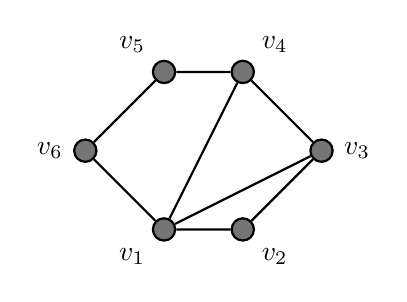
\begin{tikzpicture}[thick]
			\node[vertice, label={225:$v_1$}] (v1) at ( 0,0) {};	
			\node[vertice, label={-45:$v_2$}] (v2) at ( 1,0) {};	
			\node[vertice, label={360:$v_3$}] (v3) at ( 2,1) {};	
			\node[vertice, label={045:$v_4$}] (v4) at ( 1,2) {};	
			\node[vertice, label={135:$v_5$}] (v5) at ( 0,2) {};	
			\node[vertice, label={180:$v_6$}] (v6) at (-1,1) {};	
			\path[draw=black] (v1)--(v2)--(v3)--(v4)--(v5)--(v6)--(v1)--(v4)(v1)--(v3);
		\end{tikzpicture}\\$G$
		\end{center}
		\end{minipage}
		\begin{minipage}[b]{0.3\textwidth}
		\begin{center}
		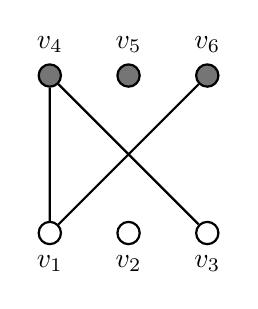
\begin{tikzpicture}[thick]
			\node[vertice, label={-90:$v_1$}, fill=white] (v1) at (0,0) {};	
			\node[vertice, label={-90:$v_2$}, fill=white] (v2) at (1,0) {};	
			\node[vertice, label={-90:$v_3$}, fill=white] (v3) at (2,0) {};	
			\node[vertice, label={090:$v_4$}] (v4) at (0,2) {};	
			\node[vertice, label={090:$v_5$}] (v5) at (1,2) {};	
			\node[vertice, label={090:$v_6$}] (v6) at (2,2) {};	
			\path[draw=black] (v1)(v2)(v3)--(v4)(v5)(v6)--(v1)--(v4)(v1)(v3);
		\end{tikzpicture}\\$H$
		\end{center}
		\end{minipage}
		\begin{minipage}[b]{0.3\textwidth}
		\begin{center}
		Chuyển cạnh $v_5$ sang phía còn lại:
		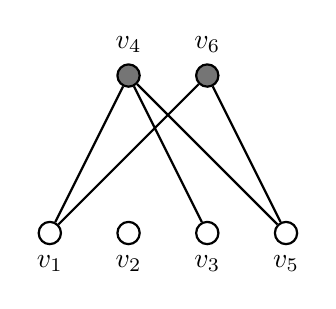
\begin{tikzpicture}[thick]
			\node[vertice, label={-90:$v_1$}, fill=white] (v1) at (0,0) {};	
			\node[vertice, label={-90:$v_2$}, fill=white] (v2) at (1,0) {};	
			\node[vertice, label={-90:$v_3$}, fill=white] (v3) at (2,0) {};	
			\node[vertice, label={-90:$v_5$}, fill=white] (v5) at (3,0) {};	
			\node[vertice, label={090:$v_4$}] (v4) at (1,2) {};	
			\node[vertice, label={090:$v_6$}] (v6) at (2,2) {};	
			\path[draw=black] (v1)(v2)(v3)--(v4)--(v5)--(v6)--(v1)--(v4)(v1)(v3);
		\end{tikzpicture}\\$H'$
		\end{center}
		\end{minipage}
	\end{center}
	\caption{Minh họa cho định lý \ref{theo:sub_bigraph}}
	\label{fig:minh_hoa_cho_dinh_ly_sub_bigraph}
\end{figure}



\section{Một số mệnh đề}
\begin{proposition}
	\label{prop:number_of_n_vertice_graph} Số đồ thị đơn giản với tập đỉnh có $n$ phần tử là $2^{C_n^2}$	
	\begin{proof}
		Gọi $V$ là tập đỉnh có $n$ phần tử. Ta xây dựng các đồ thị giản đơn $G$ từ tập đỉnh $V$. Có $C^2_n$ cách chọn một cặp cạnh ở trong $V$. Với mỗi cặp cạnh, ta có 2 lựa chọn: kề nhau hoặc không kề nhau. Do đó có tổng cộng $2^{C_n^2}$ đồ thị đơn giản với $n$ đỉnh.
	\end{proof}
\end{proposition}

\begin{proposition}
	Với $n > 2$, có $2^{C_{n-1}^2}$ đồ thị đơn giản có các đỉnh $v_1$, $v_2$, $v_3, \ldots, v_n$ mà bậc của mỗi đỉnh đều chẵn.
	\begin{proof}
		Gọi tập $A$ là tập các đồ thị đơn giản mà có các đỉnh là $v_1$, $v_2$, $v_3, \ldots, v_{n-1}$, $B$ là tập các đồ thị đơn giản với các đỉnh $v_1$, $_2$, $_3,\ldots,v_n$. Theo mệnh đề \ref{prop:number_of_n_vertice_graph} ta có $\abs{A} = 2^{C_{n-1}^2}$. Ta định nghĩa ánh xạ $f:A\to B$: $f$ biến đồ thị $G \in A$ thành $H \in B$ bằng cách thêm một đỉnh $v_n$, sau đó nối $v_n$ với các đỉnh bậc lẻ của $G$. Khi đó các đỉnh bậc lẻ của $G$ cũng sẽ trở thành các đỉnh bậc chẵn trong $H$, và theo hệ quả \ref{coro:number_of_odd_degree_vertices_is_even}, bản thân $v_n$ cũng là bậc chẵn. Ngược lại, nếu lấy đồ thị $H$ bất kì thuộc $B$ và ngắt bỏ đỉnh $v_n$, ta thu được một đồ thị $G$ tương ứng thuộc $A$. Dễ thấy ngay quá trình này là nghịch đảo của quá trình trên, do đó $f$ là một song ánh. Vì $f$ là song ánh nên $\abs{B} = \abs{A} = 2^{C_{n-1}^2}$
	\end{proof}
\end{proposition}

\begin{proposition}
	Đồ thị đơn giản mà có nhiều hơn một đỉnh thì có hai đỉnh với bậc bằng nhau.
	\begin{proof}
		Trong đồ thị với $n$ đỉnh, bậc của các đỉnh nhận giá trị trong tập $\left\{0,1,2,3,\ldots,n-1\right\}$. Tuy nhiên, giá trị $0$ và $n-1$ sẽ không xuất hiện cùng một lúc vì đỉnh có bậc $n-1$ sẽ kề với mọi đỉnh, đỉnh có bậc $0$ là cô lập, 2 đỉnh như trên không thể cùng xuất hiện trong một đồ thị. Do đó, số giá trị bậc các đỉnh của $G$ luôn bé hơn $n$, theo nguyên líDirichlet, mệnh đề được chứng minh.
	\end{proof}
\end{proposition}
\begin{proposition}
	Nếu $G$ là đồ thị đơn giản với $n$ đỉnh và $\delta(G) \ge (n-1)/2$ thì $G$ liên thông.
	\begin{proof}
		Lấy 2 đỉnh $u,v \in V(G)$. Giả sử $u,v$ không kề nhau. Vì $\delta(G) \ge (n-1)/2$, sẽ có ít nhất $n-1$ cạnh để nối $u$ hoặc $v$ tới các đỉnh khác. Tuy nhiên chỉ có $n-2$ cạnh, do đó theo nguyên lí Dirichlet, sẽ có một đỉnh nào đó kề với cả $u$ và $v$. Vậy mỗi cặp đỉnh trong $G$ đều tồn tại một đường đi giữa chúng.
	\end{proof}
\end{proposition}




\printbibliography[heading=bibintoc,title={Danh mục tài liệu tham khảo}]
\end{document}
